\begin{center}
	\section{Planta de extracci\'on}
\end{center}

\noindent
\justify

La planta de extracci\'on consiste de las siguientes etapas:

\begin{itemize}
	\item Preprocesamiento
	\item Eluci\'on y filtrado
	\item Separaci\'on de sustancias
\end{itemize}

\noindent
\justify

El \textit{objetivo} de la presente investigaci\'on consiste en el planteamiento del dise\~no del sistema de eluci\'on y filtrado, enfocado en la etapa de separaci\'on de sustancias, de la planta de extracci\'on; como se aprecia en la Figura \ref{biofabrica}\footnote{Nomenclatura:
\begin{itemize}
	\item $m_v \rightarrow $ Material vegetal.
	\item $m_p \rightarrow $ Material pulverizado (mezcla entre el material vegetal con el agente dispersante).
	\item $FS \rightarrow $ Fase s\'olida. Corresponde al residuo del material pulverizado despu\'es de la extracci\'on.
	\item $FL \rightarrow $ Fase l\'iquida. Corresponde a la mezcla l\'iquida homog\'enea entre el solvente y el extracto.
\end{itemize}}

\begin{figure}[h!]
	\centering
	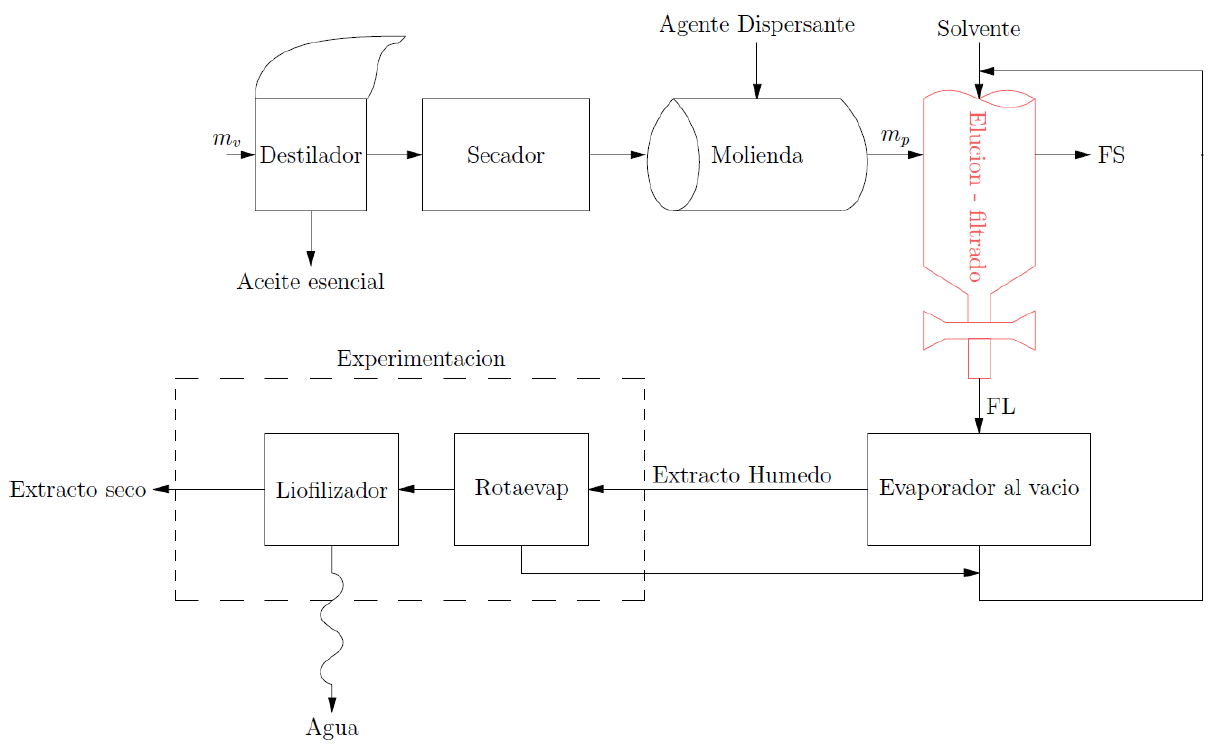
\includegraphics[width=\textwidth]{Images/planta.PNG}
	\caption{Flujo de trabajo.}
	\label{biofabrica}
\end{figure}


